% Copyright 2004 by Till Tantau <tantau@users.sourceforge.net>.
%
% In principle, this file can be redistributed and/or modified under
% the terms of the GNU Public License, version 2.
%
% However, this file is supposed to be a template to be modified
% for your own needs. For this reason, if you use this file as a
% template and not specifically distribute it as part of a another
% package/program, I grant the extra permission to freely copy and
% modify this file as you see fit and even to delete this copyright
% notice. 

\documentclass{beamer}

\usepackage{CJKutf8}
\usepackage{rotating}
\usepackage{subfigure}
\usepackage{graphicx}
\usepackage{algorithm}
\usepackage{algorithmicx}
\usepackage{amsmath}
\usepackage{amssymb}
\usepackage{algpseudocode}
\algdef{SE}[DOWHILE]{Do}{DoWhile}{\algorithmicdo}[1]{\algorithmicwhile\ #1}%


% There are many different themes available for Beamer. A comprehensive
% list with examples is given here:
% http://deic.uab.es/~iblanes/beamer_gallery/index_by_theme.html
% You can uncomment the themes below if you would like to use a different
% one:
%\usetheme{AnnArbor}
%\usetheme{Antibes}
%\usetheme{Bergen}
%\usetheme{Berkeley}
%\usetheme{Berlin}
%\usetheme{Boadilla}
%\usetheme{boxes}
%\usetheme{CambridgeUS}
%\usetheme{Copenhagen}
%\usetheme{Darmstadt}
%\usetheme{default}
%\usetheme{Frankfurt}
%\usetheme{Goettingen}
%\usetheme{Hannover}
%\usetheme{Ilmenau}
%\usetheme{JuanLesPins}
%\usetheme{Luebeck}
\usetheme{Madrid}
%\usetheme{Malmoe}
%\usetheme{Marburg}
%\usetheme{Montpellier}
%\usetheme{PaloAlto}
%\usetheme{Pittsburgh}
%\usetheme{Rochester}
%\usetheme{Singapore}
%\usetheme{Szeged}
%\usetheme{Warsaw}


% A subtitle is optional and this may be deleted
%\subtitle{Optional Subtitle}

\author{Chi-Ming~Lee}
% - Give the names in the same order as the appear in the paper.
% - Use the \inst{?} command only if the authors have different
%   affiliation.

\institute[National Tsing Hua University] % (optional, but mostly needed)
{
    Department of Electrial Engineering\\
    National Tsing Hua University
}
% - Use the \inst command only if there are several affiliations.
% - Keep it simple, no one is interested in your street address.

\date{\today}
% - Either use conference name or its abbreviation.
% - Not really informative to the audience, more for people (including
%   yourself) who are reading the slides online

%\subject{Theoretical Computer Science}
% This is only inserted into the PDF information catalog. Can be left
% out. 

% If you have a file called "university-logo-filename.xxx", where xxx
% is a graphic format that can be processed by latex or pdflatex,
% resp., then you can add a logo as follows:

% \pgfdeclareimage[height=0.5cm]{university-logo}{university-logo-filename}
% \logo{\pgfuseimage{university-logo}}

% Delete this, if you do not want the table of contents to pop up at
% the beginning of each subsection:
\AtBeginSubsection[]
{
    \begin{frame}<beamer>{Outline}
        \tableofcontents[currentsection,currentsubsection]
    \end{frame}
}

% Let's get started
\begin{document}
\begin{CJK}{UTF8}{bkai}

    \title{ DeAr: 適用於異質系統架構之高效率且彈性的數位訊號處理器設計}
    \subtitle{DeAr: An Efficient and Flexible Digital Signal Processor Design for Heterogeneous System Architecture}

    \begin{frame}
        \titlepage
    \end{frame}

    \begin{frame}{Outline}
        \tableofcontents
        % You might wish to add the option [pausesections]
    \end{frame}

    % Section and subsections will appear in the presentation overview
    % and table of contents.

    \section{Introduction}

    \subsection{Motivation}

    \begin{frame}{Motivation}
        \begin{itemize}
            \item {
                    The evolution of wireless communication standard drives the quest on a new DSP architecture.
                }
            \item {
                    LTE-A demands 10 times transmission throughput than that of LTE. As a result...
                    \begin{itemize}
                        \item {
                                More sophisticated arithmetics are needed (throughput).
                            }
                        \item {
                                Algorithms for demodulation need to evolve rapidly (flexibility).
                        }
                        \item {
                                Endurance of embedded devices still matters (power-efficiency).
                        }
                    \end{itemize}
                }
            \item {
                    Conventional DSP architectures, VLIW and ASIP, are opposite extreme cases for processor design.
                }
        \end{itemize}

        \begin{figure}
            \caption{VLIW vs ASIP: Flexibility vs power-efficiency}
            \begin{center}
                \subfigure[VLIW datapath]
                {
                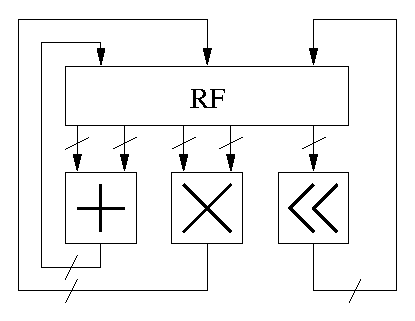
\includegraphics[width=0.2\textwidth]{./figs/vliw.eps}
                \label{fig:vliw}
            }
                \subfigure[ASIP datapath]
                {
                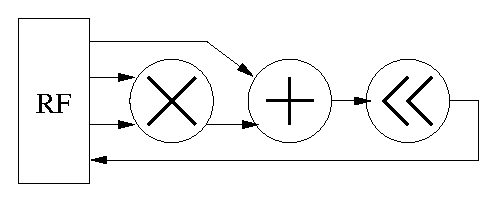
\includegraphics[width=0.3\textwidth]{./figs/cascade.eps}
                \label{fig:cascade}
            }
            \end{center}
        \end{figure}
        \begin{itemize}
            \item {
                   Achieving both of them is challenging! 
                }
        \end{itemize}
    \end{frame}

    \begin{frame}{Motivation, cont.}
        \begin{itemize}
            \item {
                    Heterogeneous computing, a system with multiple types of processors, is gaining momentum.
                    \begin{itemize}
                        \item {
                                CPU handles control-intensive tasks.
                            }
                        \item {
                                DSP, GPU and FPGA handles data-intensive tasks.
                            }
                        \end{itemize}
                }
            \item {
                    Industry standard for heterogeneous computing, \textit{Heterogeneous System Architecture} emerged in 2012.
                    \begin{itemize}
                        \item {
                                Proposed by leading semiconductor companies, AMD, ARM, MediaTek, Samsung etc, 
                            }
                        \item {
                                It has opened a new era for embedded computing platforms.
                            }
                        \end{itemize}
                }
        \end{itemize}
    \end{frame}


    \subsection{Contribution}

    \begin{frame}{Contribution}
        \begin{itemize}
            \item {
                    We propose Dual-thread Architecture (DeAr) for DSP, which achieves both power-efficiency and flexibility.
                    \begin{itemize}
                        \item {
                                The multi-issue datapath manipulating Simultaneous Multi-threading (SMT).
                            }
                        \item {
                                Multi-banked register file (RF) with implicit RF addressing.
                            }
                        \item {
                                Transport-triggered data bus for exhaustive data forwarding.
                            }
                        \end{itemize}
                }
            \item {
                    We propose a framework to integrate DeAr DSP with an HSA platform.
                    \begin{itemize}
                        \item {
                                HSA compatible system integration framework.
                            }
                        \item {
                                HSA compatible compilation framework.
                            }
                        \end{itemize}
                }
            \item{
        Compared with VLIW and ASIP respectively, DeAr saves: 
                    \begin{itemize}
                        \item {
                            20.3\%--13.1\% and 31.8\%--2.2\% of power, 36.1\%--31.5\% and 28.2\%--5.7\% of area in the 1st benchmark suit.
                            }
                        \item {
                            20.3\%--13.1\% and 31.8\%--2.2\% of power, 36.1\%--31.5\% and 28.2\%--5.7\% of area in the 2nd benchmark suit.
                            }
                        \end{itemize}
                }
        \end{itemize}
    \end{frame}

    \section{Heterogeneous System Architecture}
    \begin{frame}{HSA platform example}
        \begin{figure}[!ht] 
            \centering
            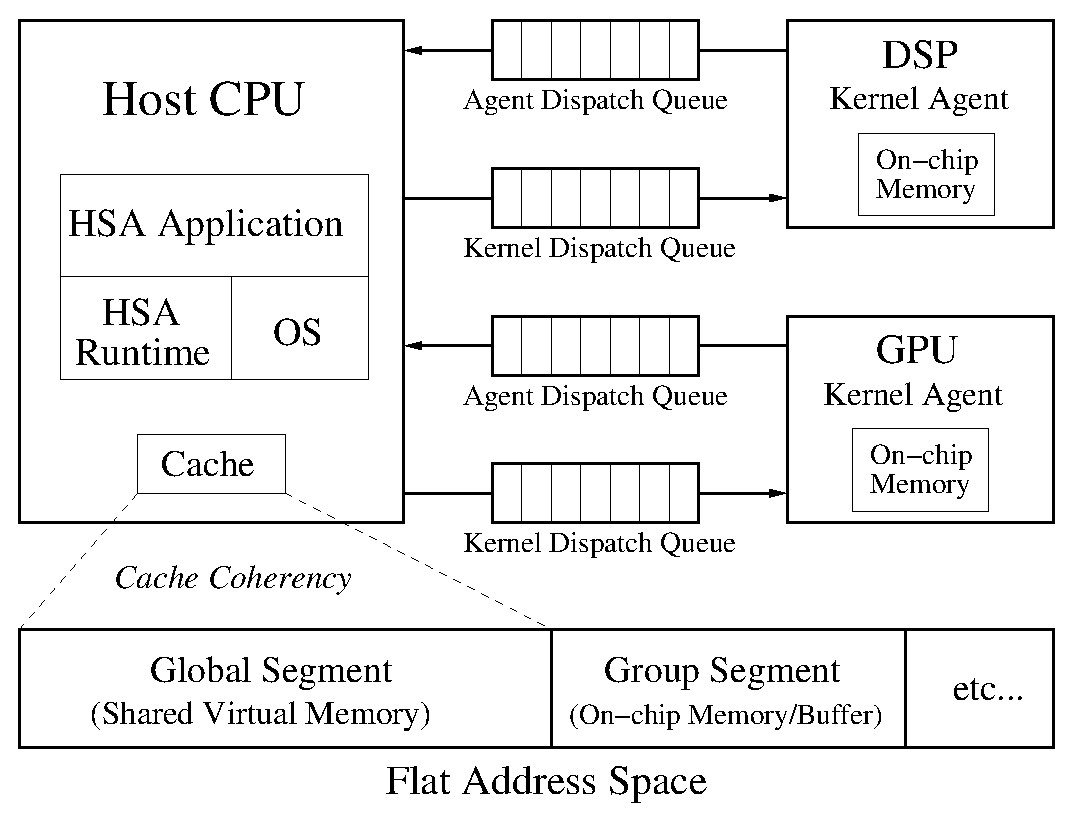
\includegraphics[width=0.8\textwidth]{./figs/systemspec.eps}
            \label{fig:systemspec}
        \end{figure}
    \end{frame}

    \begin{frame}{Execution hierarchy}
        \begin{figure}[!ht] 
            \centering
            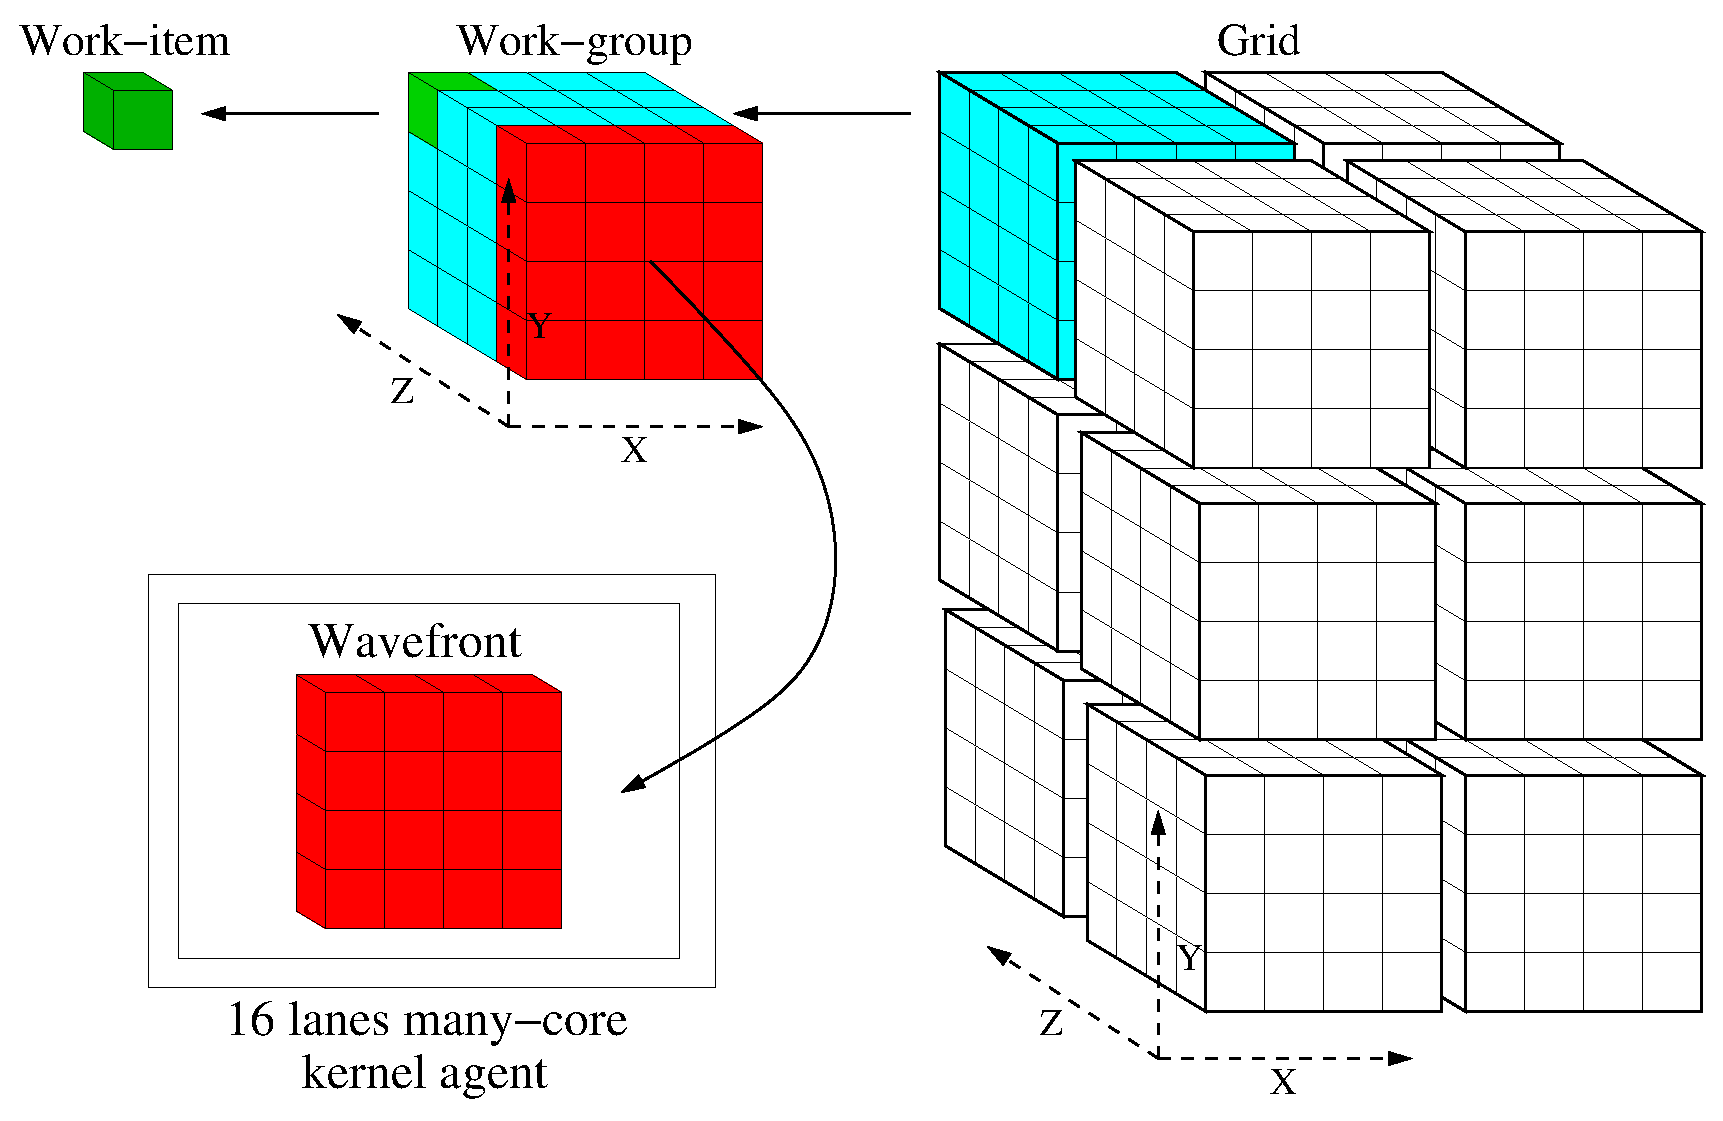
\includegraphics[width=0.8\textwidth]{./figs/grid.eps}
            \label{fig:grid}
        \end{figure}
    \end{frame}

    \begin{frame}{Software Infrastructure of HSA}
        \begin{figure}[!ht] 
            \centering
            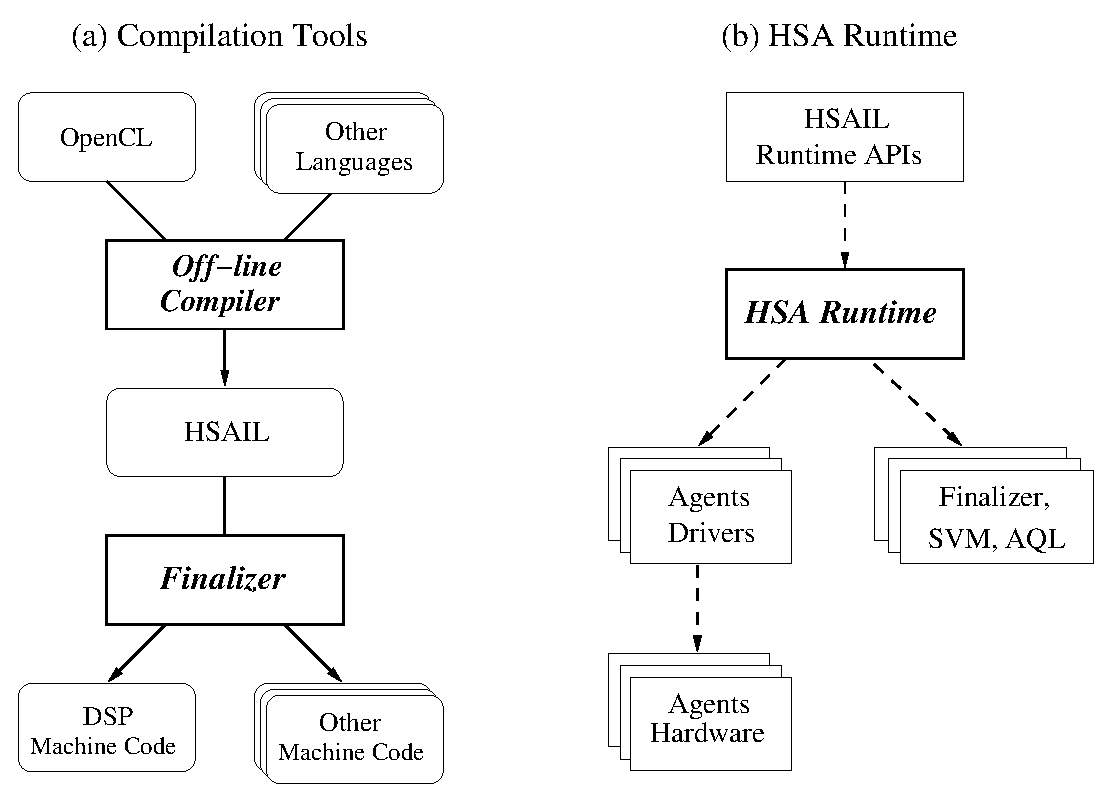
\includegraphics[width=0.8\textwidth]{./figs/swinf.eps}
            \label{fig:swinf}
        \end{figure}
    \end{frame}


    \section{Design and Implementation}

    \subsection{Concepts of DeAr}
    \begin{frame}{Concepts of DeAr}
        \begin{figure}[!ht]
            \begin{center}
                \subfigure[Execution flow of an HSA work-item]
                {
                    \label{fig:bb:1}
                    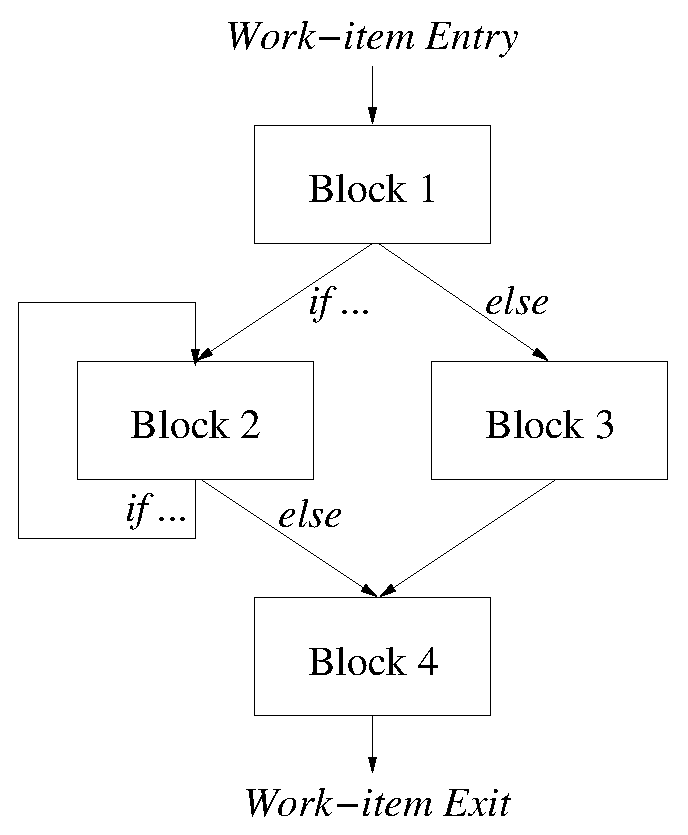
\includegraphics[width=0.3\textwidth]{figs/bb.eps}
                }
                \hfill
                \subfigure[Accelerating the execution of a Basic block]
                {
                    \label{fig:bb:2}
                    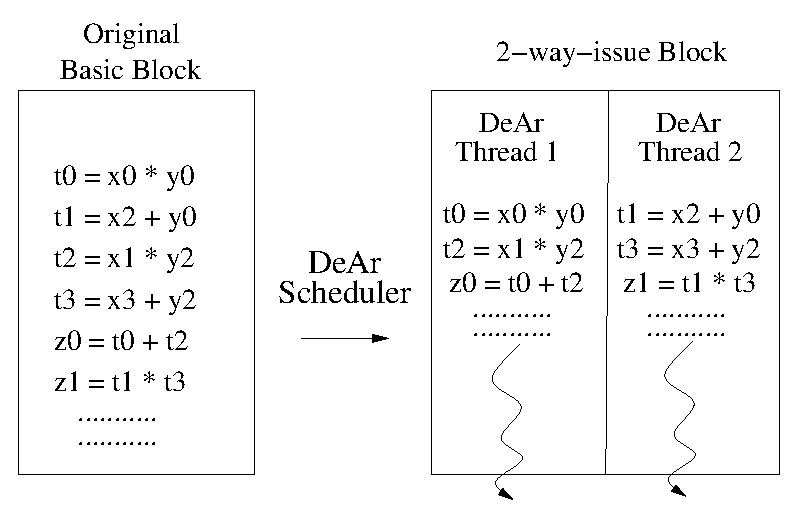
\includegraphics[width=0.55\textwidth]{figs/bb2.eps}
                }
            \end{center}
            \caption{Accelerating HSA with DeAr}
            \label{fig:bb}
        \end{figure}
    \end{frame}

    \subsection{Proposed architecture}
    \begin{frame}{Proposed architecture}
        \begin{figure}[!ht] 
            \centering
            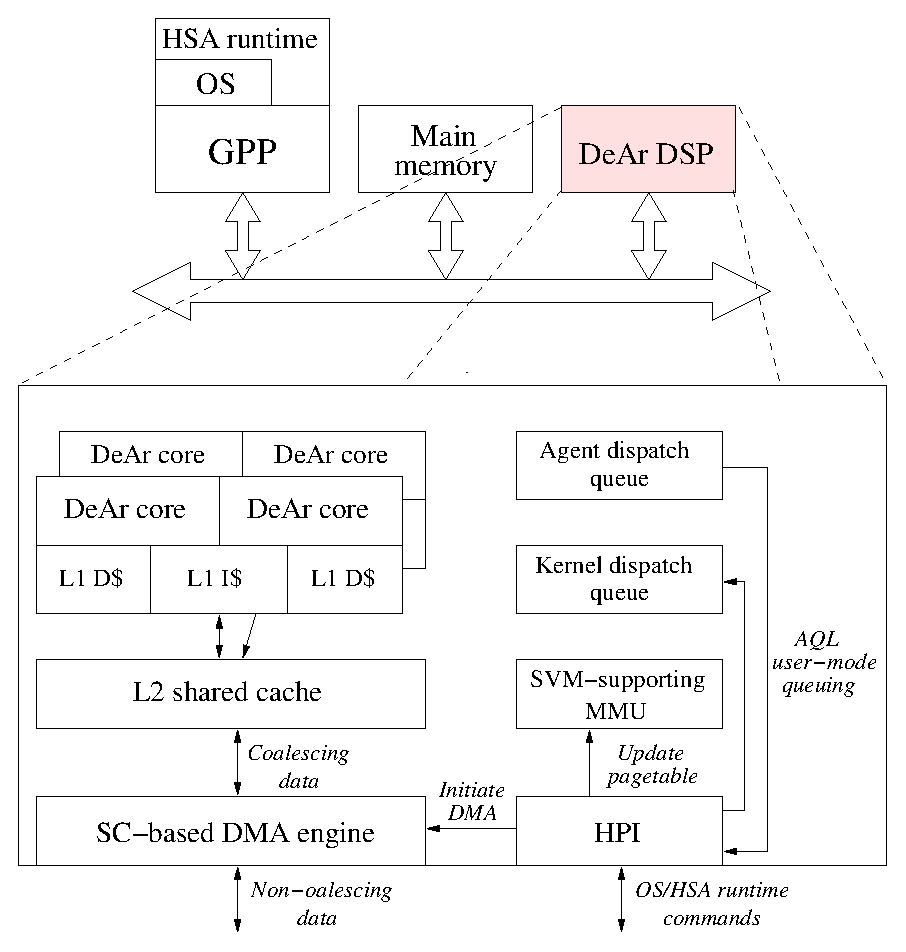
\includegraphics[width=0.5\textwidth]{./figs/archi.eps}
            \label{fig:archi}
        \end{figure}
    \end{frame}

    \begin{frame}{Proposed architecture, cont.}
        \begin{itemize}
            \item {
                    \textbf{MMU}: The host OS accesses MMU via HPI, and thus HSA SVM can be facilitated.
                }
            \item {
                    \textbf{Dispatch queues}: HSA runtime pushes (pops out) AQL-packets to (from) the kernel-dispatch queue (agent-dispatch queue) via HPI, 
                    and thus HSA user-mode queuing can be facilitated.
                }

            \item {
                    \textbf{SC}: The SC user API sends control signal to SC via HPI, 
                    and thus the data transfer and conversion fashion can be specified by the user.
                }
        \end{itemize}
    \end{frame}

    \subsection{Micro-architecture Design}
    \begin{frame}{Micro-architecture Design}
        \begin{figure}[!ht] 
            \centering
            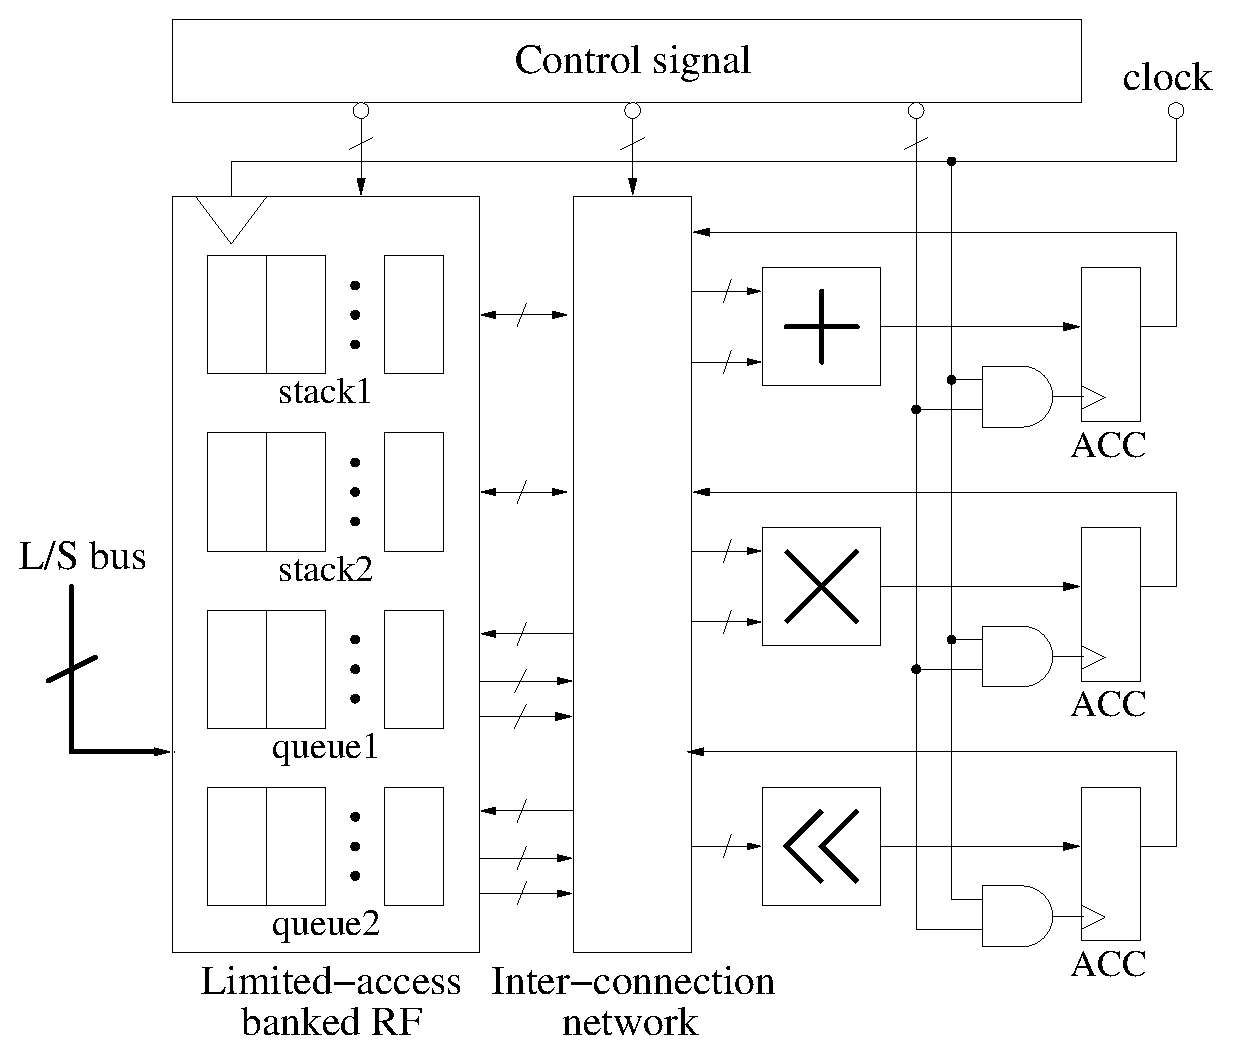
\includegraphics[width=0.6\textwidth]{./figs/micro.eps}
            \label{fig:micro}
        \end{figure}
    \end{frame}

 
    \section{Compilation}
    \subsection{HDFG}
    \begin{frame}{DFG to HDFG}
        \begin{figure}[!ht]
            \begin{center}
                \subfigure[DFG example]
                {
                    \label{fig:dfg:dfg}
                    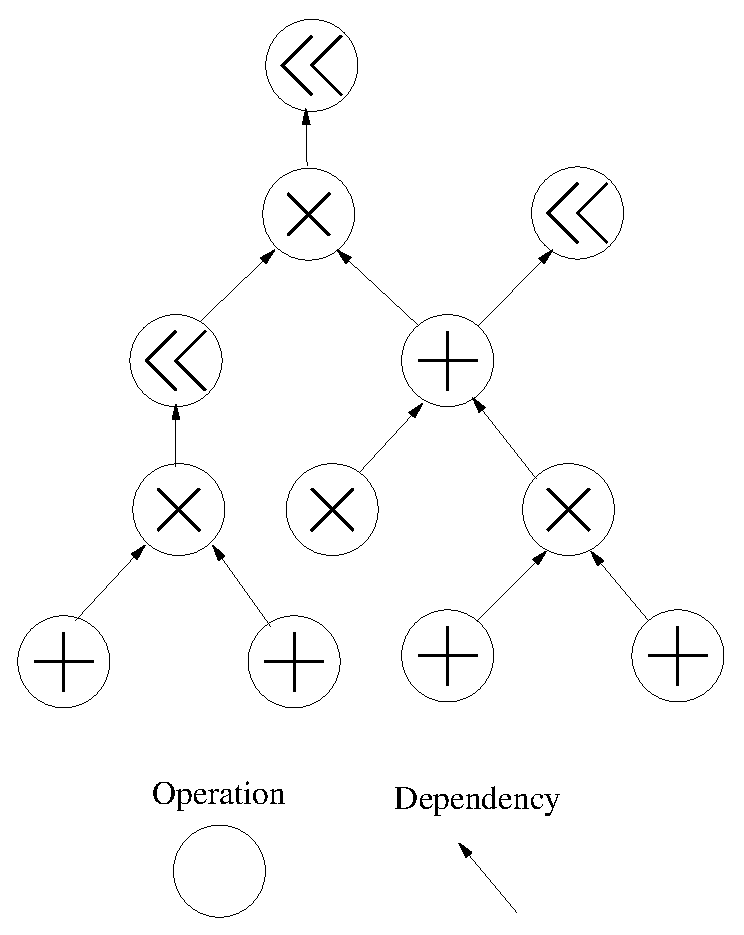
\includegraphics[width=0.4\textwidth]{figs/dfg.eps}
                }\hfill
                \subfigure[Corresponding HDFG]
                {
                    \label{fig:dfg:hdfg}
                    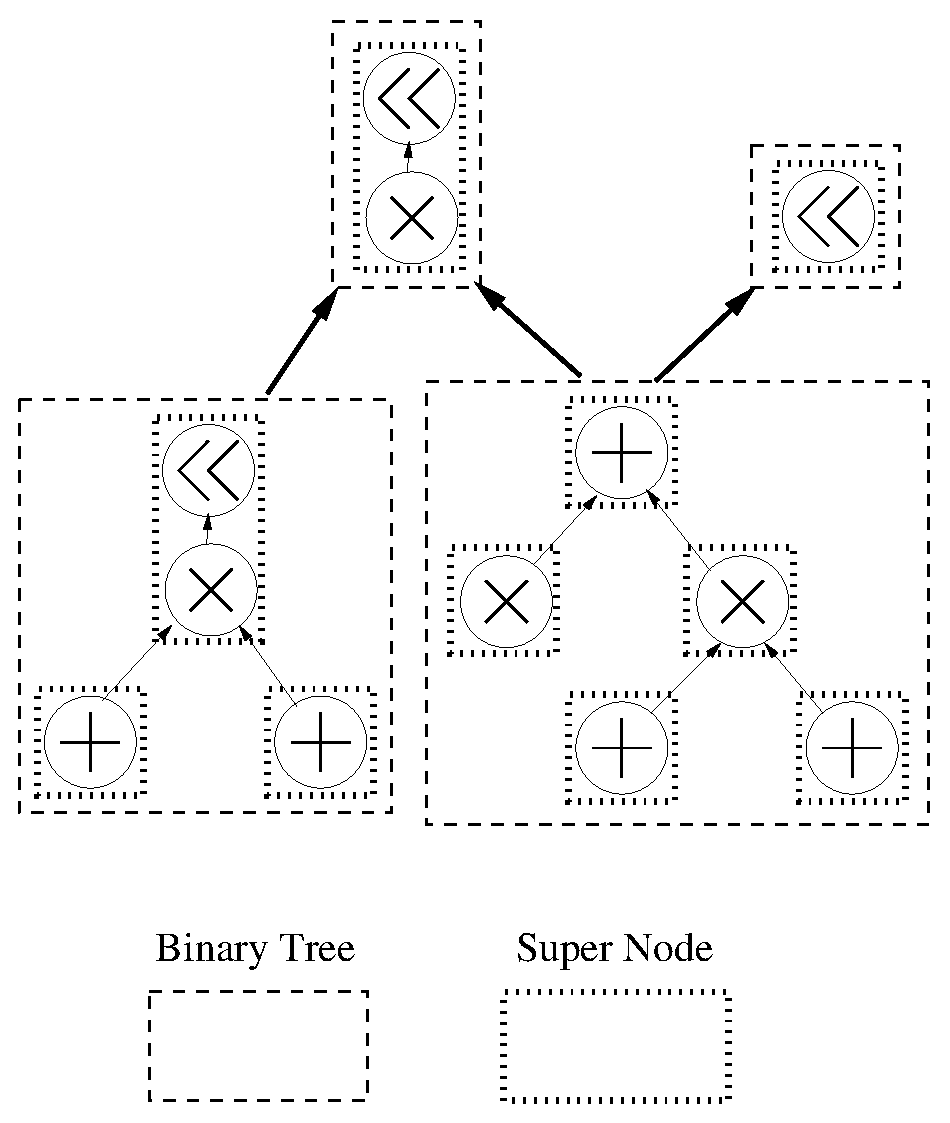
\includegraphics[width=0.4\textwidth]{figs/hdfg.eps}
                }
            \end{center}
            \label{fig:dfg}
        \end{figure}
    \end{frame}


    \subsection{HDFG-based scheduling}
    \begin{frame}{Higher-subtree-first postorder traversal sort}
        \begin{figure}[!h]
            \begin{center}
                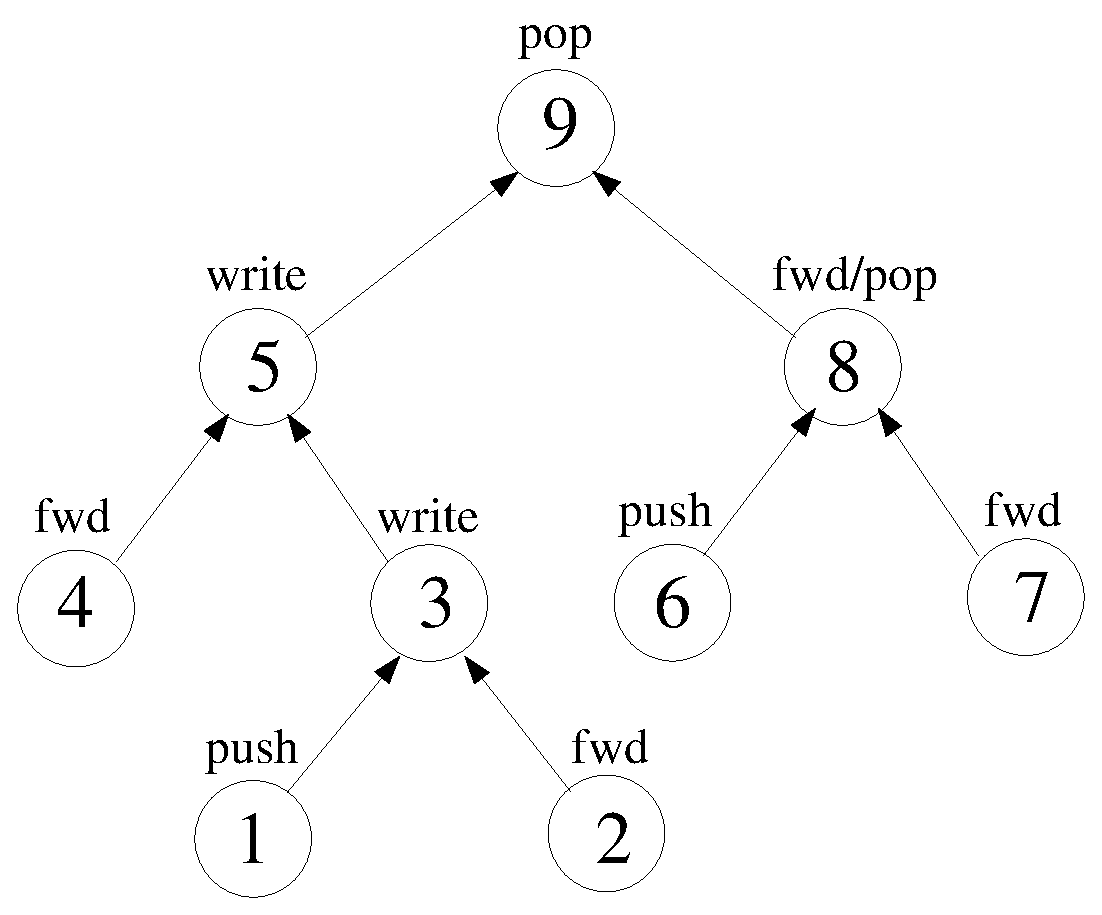
\includegraphics[width=0.6\textwidth]{figs/hfpt.eps}
            \end{center}
            \label{fig:hfpt}
        \end{figure}%
    \end{frame}

    \begin{frame}{DP-based ALU-allocation}
        \begin{figure}[!ht]
            \begin{center}
                \subfigure[Stage 1: scoring table modeling]
                {
                    \label{fig:alloc:1}
                    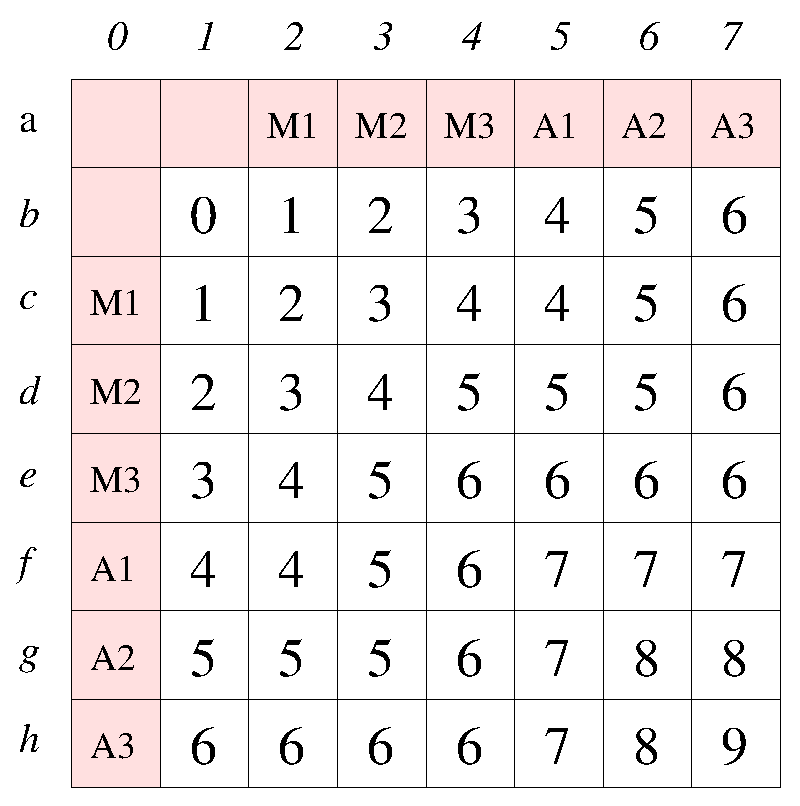
\includegraphics[width=0.3\textwidth]{figs/alloc.eps}
                }
                \hfill
                \subfigure[Stage 2: scoring table filling]
                {
                    \label{fig:alloc:2}
                    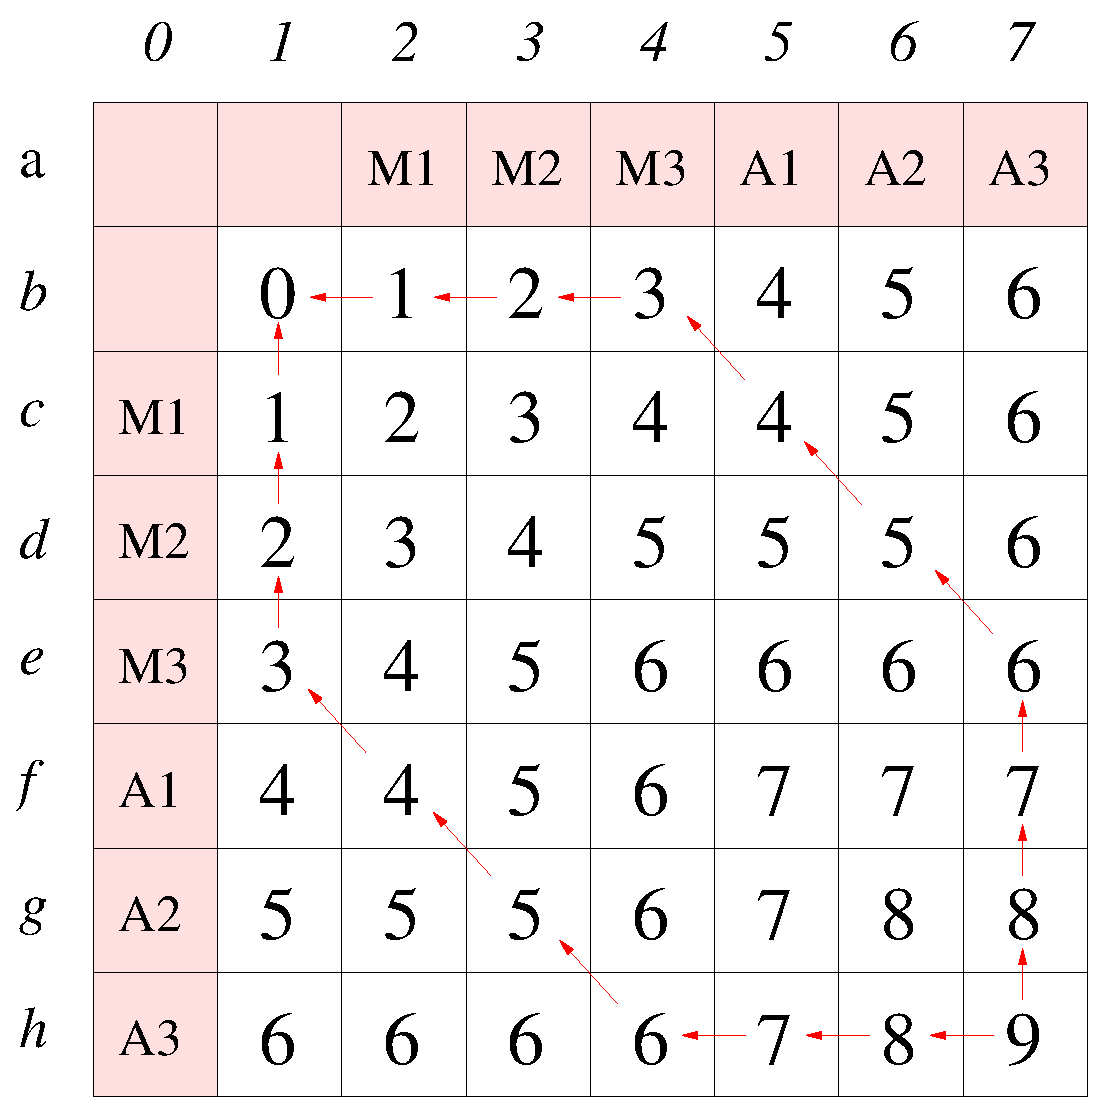
\includegraphics[width=0.3\textwidth]{figs/alloc2.eps}
                }
                \hfill
                \subfigure[Stage 3: backtracking]
                {
                    \label{fig:alloc:3}
                    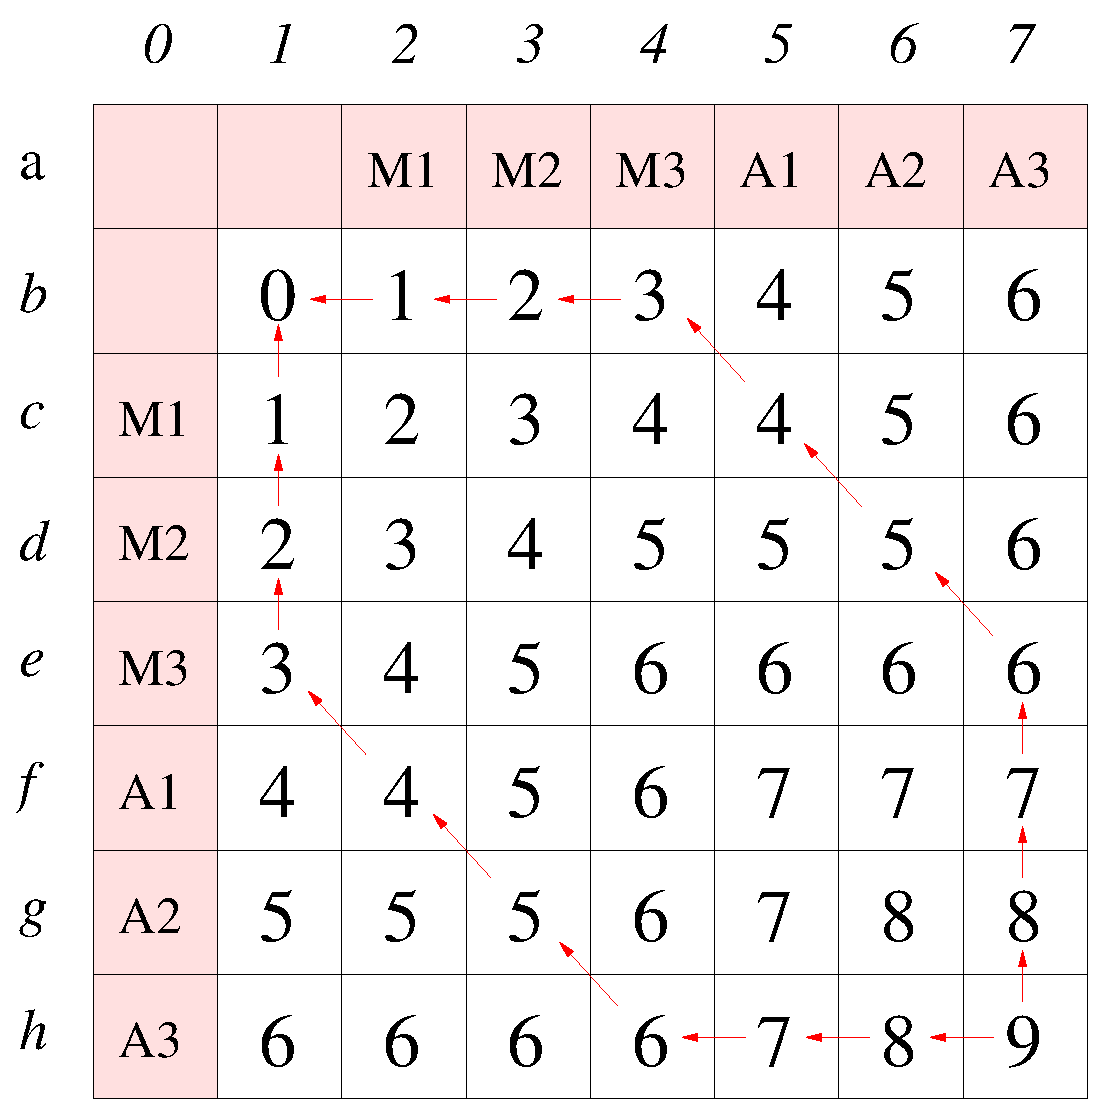
\includegraphics[width=0.3\textwidth]{figs/alloc3.eps}
                }
            \end{center}
            \label{fig:alloc}
        \end{figure}

    \end{frame}

\end{CJK}
\end{document}


